\documentclass[upright, contnum, oneside]{umemoria}
\depto{DEPARTAMENTO DE ASTRONOMÍA}
\author{PÍA GABRIELA CORTÉS ZULETA}
\title{THE TRAMOS PROJECT UPDATED: ENHANCED SAMPLE OF TRANSITING EXOPLANETS, STRATEGIES, AND ANALYSIS}
\titulo{THE TRAMOS PROJECT UPDATED: ENHANCED SAMPLE OF TRANSITING EXOPLANETS, STRATEGIES AND ANALYSIS}

\date{2019}
\fecha{2019}
\guia{PATRICIO ROJO RUBKE}

\carrera{MAGÍSTER EN CIENCIAS MENCIÓN ASTRONOMÍA}
\memoria{TESIS PARA OPTAR AL GRADO DE}
\comision{}

% ----------------------------------------------------------------------
% Configuracion temporal
% ----------------------------------------------------------------------
%\usepackage{minted}
\usepackage[colorinlistoftodos]{todonotes}
%\usepackage{physics}

\usepackage{amsmath}
\usepackage{amssymb}
%\usepackage{amsthm}
\usepackage{amsfonts}
\usepackage{dsfont}
%\usepackage{pifont}% http://ctan.org/pkg/pifont
\newcommand{\cmark}{\ding{52}}%
\newcommand{\xmark}{\ding{56}}%
\usepackage{etoolbox}	% robustify command

%%%%%%%%%%%%%%%%%%%%%%%%%%%%%%%%%%%%%%%%%%%%%%%%%%%%%%%%%%%%%%%%%%%%%%%%%%%%%%%%
% General utilities
%%%%%%%%%%%%%%%%%%%%%%%%%%%%%%%%%%%%%%%%%%%%%%%%%%%%%%%%%%%%%%%%%%%%%%%%%%%%%%%%

% etal command
\newcommand{\etal}{\emph{et al.}\ }

%%%%%%%%%%%%%%%%%%%%%%%%%%%%%%%%%%%%%%%%%%%%%%%%%%%%%%%%%%%%%%%%%%%%%%%%%%%%%%%%
% Probability
%%%%%%%%%%%%%%%%%%%%%%%%%%%%%%%%%%%%%%%%%%%%%%%%%%%%%%%%%%%%%%%%%%%%%%%%%%%%%%%%

\newcommand{\prob}[1]{\mathrm{P}\left( #1 \right)}

% Gaussian
\newcommand{\DistributionGaussian}[2]{\mathcal{N}(#1,#2)}

% Noisy format (tilde)
\newcommand{\noisy}[1]{\tilde{#1}}

% Estimate (hat upper)
\newcommand{\estimate}[1]{\hat{#1}}

% Mahalanobis norm
\newcommand{\mahalanobisNorm}[2]{\lVert{#1}\rVert^{2}_{#2}}

% Huber norm
\newcommand{\huberNorm}[2]{\rho_h\left(#1\right)_{#2}}

% Covariance of (text version)
\newcommand{\Cov}[1]{\mathrm{Cov}\!\left(#1\right)}

%%%%%%%%%%%%%%%%%%%%%%%%%%%%%%%%%%%%%%%%%%%%%%%%%%%%%%%%%%%%%%%%%%%%%%%%%%%%%%%%
% Optimization
%%%%%%%%%%%%%%%%%%%%%%%%%%%%%%%%%%%%%%%%%%%%%%%%%%%%%%%%%%%%%%%%%%%%%%%%%%%%%%%%

% Optimum notation (superscript asterisk)
\newcommand{\optimum}[1]{{#1}^{*}}

% partial derivative
\newcommand{\diffPartial}[2]{\displaystyle \frac{\partial #1}{\partial #2}}

% argmin
\newcommand{\argmin}{\operatornamewithlimits{arg\,min}}
% argmax
\newcommand{\argmax}{\operatornamewithlimits{arg\,max}}

%%%%%%%%%%%%%%%%%%%%%%%%%%%%%%%%%%%%%%%%%%%%%%%%%%%%%%%%%%%%%%%%%%%%%%%%%%%%%%%%
% Geometry
%%%%%%%%%%%%%%%%%%%%%%%%%%%%%%%%%%%%%%%%%%%%%%%%%%%%%%%%%%%%%%%%%%%%%%%%%%%%%%%%

% Euclidean space
\newcommand{\Rn}[1]{\mathbb{R}^{#1}}

% Trace
\newcommand{\traceNew}[1]{\mathrm{tr}(#1)}

% skew symmetric matrix
\newcommand{\matrixSkew}[3]{
	\begin{bmatrix}
		  0 & -#3 &  #2 \\
		 #3 &   0 & -#1 \\
		-#2 &  #1 &   0
	\end{bmatrix}
	}

% Transformation Matrix
\newcommand{\matrixRigidBody}[2]{
	\left[
	\begin{array}{cc}
		#1  &  #2 \\
		0_{1\times3} &   1
	\end{array}
	\right]
}

% Extrinsic Matrix
\newcommand{\matrixExtrinsic}[2]{
	\left[
	\begin{array}{c|c}
		#1 & #2
	\end{array}
	\right]
}

% camera projection model
\newcommand{\cameraProjectionModel}[2]{
	\notatVector{\pi}({#1}, {#2})
}

% camera depth map model (LSD SLAM)
\newcommand{\cameraDepthMapModel}[3]{
	\notatVector{\pi}({#1}, {#2}, {#3})
}

% inverse camera projection model
\newcommand{\inverseCameraProjectionModel}[3]{
	\notatVector{\pi}^{-1}({#1}, {#2}, {#3})
}



% Frame
% subarrow used in the frame notation
\newcommand{\subarrow}[1]{
	\mathord{
		\renewcommand{\arraystretch}{0}
		\begin{array}[t]{@{}c@{}l@{}}
			#1\\[2pt]
			\hspace{-2pt}\scriptstyle\longrightarrow
		\end{array}
		\kern\scriptspace
	}
}
% frame definition
\newcommand{\notatFrame}[1]{\subarrow{\mathcal{F}}{}_{\scriptscriptstyle #1}}

% Format for matrices, vectors, scalars, homogeneous points and manifolds
% Single letters
\newcommand{\notatMatrix}[1]{\boldsymbol{\mathrm{#1}}}
\newcommand{\notatVector}[1]{\boldsymbol{\mathrm{#1}}}
\newcommand{\notatScalar}[1]{{#1}}
\newcommand{\notatHomog}[1]{\boldsymbol{{#1}}}
\newcommand{\notatManifold}[1]{\mathcal{\MakeUppercase{#1}}}

% Letters with right subscript
\newcommand{\notationMatrix}[2]{\boldsymbol{\mathrm{#1}}_{\scriptscriptstyle #2}}
\newcommand{\notationVector}[2]{\boldsymbol{\mathrm{#1}}_{\scriptscriptstyle #2}}
\newcommand{\notationScalar}[2]{{#1}_{\scriptscriptstyle #2}}
\newcommand{\notationHomog}[2]{\boldsymbol{{#1}}_{\scriptscriptstyle #2}}
\newcommand{\notationManifold}[2]{\mathcal{\MakeUppercase{#1}}_{\scriptscriptstyle #2}}

% Letters with left and right subscript
\newcommand{\notationMatrixFrame}[3]{{\scriptscriptstyle_#2}\boldsymbol{\mathrm{#1}}_{\scriptscriptstyle #3}}
\newcommand{\notationVectorFrame}[3]{{\scriptscriptstyle_#2} \boldsymbol{ \mathrm{#1}}_{\scriptscriptstyle #3}}
\newcommand{\notationScalarFrame}[3]{{\scriptscriptstyle_#2}{#1}_{\scriptscriptstyle #3}}
\newcommand{\notationHomogFrame}[3]{{\scriptscriptstyle_#2}\boldsymbol{{#1}}_{\scriptscriptstyle #3}}

% robustify enables to use the previous definitions within captions and stuff
\robustify{\notatFrame}
\robustify{\notatMatrix}
\robustify{\notatVector}
\robustify{\notatScalar}
\robustify{\notatHomog}
\robustify{\notationMatrix}
\robustify{\notationVector}
\robustify{\notationScalar}
\robustify{\notationHomog}
\robustify{\notationMatrixFrame}
\robustify{\notationVectorFrame}
\robustify{\notationScalarFrame}
\robustify{\notationHomogFrame}

%%%%%%%%%%%%%%%%%%%%%%%%%%%%%%%%%%%%%%%%%%%%%%%%%%%%%%%%%%%%%%%%%%%%%%%%%%%%%%%%
% Lie Groups
%%%%%%%%%%%%%%%%%%%%%%%%%%%%%%%%%%%%%%%%%%%%%%%%%%%%%%%%%%%%%%%%%%%%%%%%%%%%%%%%

% Lie Groups
\newcommand{\hatop}[1]{#1^{\wedge}}
\newcommand{\veeop}[1]{#1^{\vee}}

\newcommand{\liebracket}[2]{\left[ #1, #2\right]}

% GL(n)
\newcommand{\GLN}{\mathrm{GL(N)}}

% SO(2)
\newcommand{\sotwo}{\mathfrak{so}(2)}
\newcommand{\SOtwo}{\mathrm{SO(2)}}

% SO(3)
\newcommand{\sothree}{\mathfrak{so}(3)}
\newcommand{\SOthree}{\mathrm{SO(3)}}

% SO(N)
\newcommand{\soN}{\mathfrak{so}(N)}
\newcommand{\SON}{\mathrm{SO(N)}}

% SE(3)
\newcommand{\sethree}{\mathfrak{se}(3)}
\newcommand{\SEthree}{\mathrm{SE(3)}}

% SE(N)
\newcommand{\seN}{\mathfrak{se}(N)}
\newcommand{\SEN}{\mathrm{SE(N)}}

% Sim(3)
\newcommand{\simthree}{\mathfrak{sim}(3)}
\newcommand{\Simthree}{\mathrm{Sim(3)}}

% Generic exponential and logarithm map (using the capitalized version of Forster et al. (2015))
\newcommand{\Expmap}[1]{\mathrm{Exp}\left(#1\right)}
\newcommand{\expmap}[1]{\mathrm{exp}\left(#1\right)}
\newcommand{\Logmap}[1]{\mathrm{Log}\left(#1\right)}
\newcommand{\logmap}[1]{\mathrm{log}\left(#1\right)}

% SO(3) exponential and logarithm maps
\newcommand{\ExpmapSOthree}[1]{\mathrm{Exp}_{\SOthree}\left(#1\right)}
\newcommand{\expmapSOthree}[1]{\mathrm{exp}_{\SOthree}\left(#1\right)}
\newcommand{\LogmapSOthree}[1]{\mathrm{Log}_{\SOthree}\left(#1\right)}
\newcommand{\logmapSOthree}[1]{\mathrm{log}_{\SOthree}\left(#1\right)}

% SE(3) exponential and logarithm maps
\newcommand{\ExpmapSEthree}[1]{\mathrm{Exp}_{\SEthree}\left(#1\right)}
\newcommand{\expmapSEthree}[1]{\mathrm{exp}_{\SEthree}\left(#1\right)}
\newcommand{\LogmapSEthree}[1]{\mathrm{Log}_{\SEthree}\left(#1\right)}
\newcommand{\logmapSEthree}[1]{\mathrm{log}_{\SEthree}\left(#1\right)}

% Generic adjoint
\newcommand{\adjop}[1]{\mathrm{ad}\left(#1\right)}
\newcommand{\Adjop}[1]{\mathrm{Ad}\left(#1\right)}

% Generic Right and Left jacobian
\newcommand{\JacR}[1]{\mathit{J}_{r} \left( #1 \right)}
\newcommand{\JacInvR}[1]{\mathit{J}_{r}^{-1} \left( #1 \right)}
\newcommand{\JacL}[1]{\mathit{J}_{l} \left( #1 \right) }
\newcommand{\JacInvL}[1]{\mathit{J}_{l}^{-1} \left( #1 \right)}

% Barfoot's operators (Barfoot & Furgale, 2014)
\newcommand{\barfootOpA}[1]{\langle\!\langle #1 \rangle\!\rangle}
\newcommand{\barfootOpAB}[2]{\langle\!\langle #1, #2 \rangle\!\rangle}

\newcommand{\adjhat}[1]{{#1}^{\curlywedge}}
\newcommand{\adjvee}[1]{{#1}^{\curlyvee}}

%%%%%%%%%%%%%%%%%%%%%%%%%%%%%%%%%%%%%%%%%%%%%%%%%%%%%%%%%%%%%%%%%%%%%%%%%%%%%%%%
% Other stuff
%%%%%%%%%%%%%%%%%%%%%%%%%%%%%%%%%%%%%%%%%%%%%%%%%%%%%%%%%%%%%%%%%%%%%%%%%%%%%%%%

% image intensity norm
\newcommand{\imageIntensity}[2]{I_{#1} \left( #2 \right)}

\newcommand{\getZ}[1]{\boldsymbol{\mathsf{Z}}\left(#1\right)}

% matrix spacing adjustments
% usage: 
% \begin{pmatrix}[1.5]
% ...
% \end{pmatrix}

\makeatletter
\renewcommand*\env@matrix[1][\arraystretch]{%
	\edef\arraystretch{#1}%
	\hskip -\arraycolsep
	\let\@ifnextchar\new@ifnextchar
	\array{*\c@MaxMatrixCols c}}
\makeatother

% table stuff
\newcommand{\cell}[1]{\begin{tabular}{@{}l@{}}#1\end{tabular}}

% colors
\usepackage{color}
\usepackage{colortbl}
\definecolor{ColorLightCyan}{rgb}{0.88,1,1}
\definecolor{ColorLightTurquoise}{rgb}{0.5, 1, 0.8}



% anexos
% arreglo de: https://tex.stackexchange.com/a/260486
\usepackage{etoolbox}
\usepackage[toc]{appendix}
\makeatletter
\appto{\appendices}{\def\Hy@chapapp{Appendix}}
\makeatother

\usepackage{stackengine}

\usepackage{tabulary}

\renewcommand{\appendixtocname}{Apéndices}
\renewcommand{\appendixpagename}{Apéndices}

% configuracion de captions
\captionsetup{font=small}
\captionsetup[sub]{font=small}

\usepackage{amssymb}% http://ctan.org/pkg/amssymb
\usepackage{pifont}% http://ctan.org/pkg/pifont

% tabla con nota abajo
\usepackage[flushleft]{threeparttable} % http://ctan.org/pkg/threeparttable
% permite ajustar el tamaño de tablas y otros objetos
\usepackage{adjustbox}

% tabla de contenidos por capitulo
%\usepackage{minitoc}

% para incluir paginas adicionales con algun objeto
\usepackage{afterpage}
\usepackage{pdflscape}

% subcaptions
\usepackage{subcaption}
\usepackage{caption}

% alignment of vectors and matrices
\usepackage{mathtools}

\usepackage{natbib}

\begin{document}

% ----------------------------------------------------------------------
% Portada
% ----------------------------------------------------------------------
\frontmatter
\maketitle

% TODO list
%\todototoc
%\listoftodos


% ----------------------------------------------------------------------
% Resumen
% ----------------------------------------------------------------------
\begin{resumen}


\end{resumen}

%\begin{abstract}
	
%\end{abstract}



% ----------------------------------------------------------------------
% Dedicatoria
% ----------------------------------------------------------------------
\begin{dedicatoria} % opcional
A mis padres.
\end{dedicatoria}


% ----------------------------------------------------------------------
% Agradecimientos
% ----------------------------------------------------------------------
\begin{thanks} % opcional

Quiero agradecer en primer lugar a mis padres, quienes han sido mi apoyo fundamental tanto emocional como económico todos estos años (desde que nací). Gracias por nunca cortarme las alas, darme la libertad de soñar en grande y recogerme cada vez que me caí (literal y metafóricamente).

También quiero agradecer a mi profe guía, Pato Rojo, por la confianza de pasarme TraMoS y la libertad creativa que tuve para desarrollar este proyecto. Gracias por el apoyo y las enseñanzas estos años, me siento mucho más cerca de ser una astrónoma.

A todas las amigas y amigos que me acompañaron en este largo proceso. La oficina de los Calan-bozos se volvió una zona de comfort para mi y agradezco todos los momentos que pasamos juntos en este inhóspito lugar llamado Calán. A mis amigas de Beauchef, que nos hemos acompañado desde el primer día (casi) del Plan Común y que siempre me dieron ánimos y me apoyaron en los momentos difíciles. A Pierina, mi amiga de la vida, que aunque el universo se encarga de separarnos la amistad sigue intacta como hace catorce (?) años. A las Cazadoras de Estrellas, agredezco haber sido partícipe de este proyecto tan maravilloso que solo me dio alegrías. Sé que seguirán creciendo y motivando a más niñas a ser científicas.

A Matías, por todo tu apoyo y amor incodicional todos estos años. Por ayudarme a pararme cada vez que me caí, darme confianza las veces que ya no creía en mi misma y por escucharme atento con todas mis dudas existenciales. Gracias por ser mi fan número 1 siempre.

A Bibi, la compañera gatuna que apareció en mi vida solo para darme suavidad, ronroneos y tranquilidad. 

\end{thanks}

\addcontentsline{toc}{chapter}{Agradecimientos}
\cleardoublepage

% ----------------------------------------------------------------------
% Índice, tablas y figuras
% ----------------------------------------------------------------------
\cleardoublepage
\tableofcontents


\cleardoublepage
\addcontentsline{toc}{chapter}{List of Tables}
\listoftables

\cleardoublepage
\addcontentsline{toc}{chapter}{List of Figures}
\listoffigures


%\begin{acronyms}
	\renewcommand\arraystretch{1.5}
	\begin{center}
		%\begin{tabulary}{0.9\textwidth}{RCL}
		\begin{tabular}{r p{12cm}}
			\textbf{BA} 					& Bundle Adjustment
			\\
			\textbf{DARPA} 					& Defense Advanced Research Projects Agency
			\\
			\textbf{DIE} 					& Departamento de Ingeniería Eléctrica
			\\
			\textbf{DRC} 					& DARPA Robotics Challenge
			\\
			\textbf{KF} 					& Kalman Filter
			\\
			\textbf{EKF} 					& Extended Kalman Filter
			\\
			\textbf{FCFM} 					& Facultad de Ciencias Físicas y Matemáticas
			\\
			\textbf{IMU} 					& Inertial Measurement Unit
			\\
			\textbf{ICRA} 					& International Conference on Robotics and Automation
			\\ 
			\textbf{IROS} 					& International Conference on Intelligent Robots and Systems
			\\ 
			\textbf{LIDAR} 					& LIght Detection And Ranging
			\\
			\textbf{MAP} 					& Maximum a Posteriori
			\\ 
			\textbf{NASA} 					& National Aeronautics and Space Agency
			\\ 
			\textbf{PF} 					& Particle Filter
			\\
			\textbf{PTAM} 					& Parallel Tracking and Mapping
			\\
			\textbf{RANSAC} 				& RANdom SAmple Consensus
			\\
			\textbf{RMSE} 					& Root Mean Square Error
			\\ 
			\textbf{ROS} 					& Robot Operating System
			\\ 
			\textbf{SLAM} 					& Simultaneous Localization and Mapping
			\\
			\textbf{SVD} 					& Singular Value Decomposition
			\\
			\textbf{TSIF} 					& Two-State Implicit Filter
			\\
			\textbf{UNAB} 					& Universidad Andrés Bello
			\\ 
		\end{tabular} 
		%\end{tabulary} 
	\end{center}
	
\end{acronyms}

%\addcontentsline{toc}{chapter}{Acrónimos}

%\begin{notation}
\renewcommand\arraystretch{1.5}

\section*{Geometría básica}
\begin{center}
	%\begin{tabulary}{0.9\textwidth}{RCL}
	\begin{tabular}{l c p{12cm}}
		$\Rn{N}$ 							& : & Espacio euclideano de dimension $N$.
		\\ 
		$\notatScalar{p}$ 					& : & Valor escalar.
		\\ 
		$\notatVector{p}$ 					& : & Vector real.
		\\
		$\notatHomog{p}$ 					& : & Vector en coordenadas homogéneas.
		\\
		$\notatMatrix{A}$ 					& : & Matriz real.
		\\
		$\notatMatrix{I}$ 					& : & Matriz identidad (dimensión dependiente del contexto).
		\\
		$\notatMatrix{0}$					& : & Matriz de ceros (dimensión dependiente del contexto).
		\\
		$\notatFrame{A}$					& : & Sistema de referencia o \emph{frame} $A$.
		\\
		$\notationMatrixFrame{T}{C}{AB}$			& : & Matriz de transformación de $4\times4$ que transforma del sistema de coordenadas $\notatFrame{A}$ al $\notatFrame{B}$, definido en $\notatFrame{C}$.
		\\
		$\hatop{\left(\cdot\right)}$			& : & Operador sombrero o \emph{hat}.
		\\
		$\veeop{\left(\cdot\right)}$			& : & Operador \emph{vee}.
		\\
	\end{tabular} 
	%\end{tabulary} 
\end{center}

\section*{Estadística y optimización}
\begin{center}
	%\begin{tabulary}{0.9\textwidth}{RCL}
	\begin{tabular}{l c p{12cm}}
		$\notatMatrix{\Sigma}$							& : & Matriz de covarianza.
		\\
		$\notatMatrix{\Omega}$							& : & Matriz de información, $\notatMatrix{\Omega} = \notatMatrix{\Sigma}^{-1}$.
		\\
		$\mahalanobisNorm{\cdot}{\notatMatrix{\Omega}}$	& : & Distancia de Mahalanobis con matriz de información $\notatMatrix{\Omega}$.
		\\
		$\mahalanobisNorm{\cdot}{\notatMatrix{\Sigma}}$	& : & Distancia de Mahalanobis con matriz de covarianza $\notatMatrix{\Sigma}$.
		\\
		$\huberNorm{\cdot}{\notatMatrix{\Omega}}$		& : & Distancia de Mahalanobis con kernel robusto Huber y matriz de información $\notatMatrix{\Omega}$		
		\\
		$\huberNorm{\cdot}{\notatMatrix{\Sigma}}$		& : & Distancia de Mahalanobis con kernel robusto Huber y matriz de covarianza $\notatMatrix{\Sigma}$.
		\\
		$\noisy{\left(\cdot\right)}$			& : & Distribución de probabilidad. Variable con ruido.
		\\
		$\optimum{\left(\cdot\right)}$			& : & Variable óptima, solución de un proceso de optimización.
	\end{tabular} 
	%\end{tabulary} 
\end{center}

\section*{Variedades y Grupos de Lie}
\begin{center}
	%\begin{tabulary}{0.9\textwidth}{RCL}
	\begin{tabular}{l c p{12cm}}
		$\notationManifold{M}{\notatManifold{x}}$ 	& : & Variedad o \emph{manifold}.
		\\ 
		$\notatManifold{X},\notatManifold{Z}$ 				& : & Elemento de la variedad diferenciable $\notationManifold{M}{\notatManifold{x}}, \notationManifold{M}{\notatManifold{z}}$.
		\\
		$\boxplus$ 				& : & Operador aditivo de una variedad. diferenciable $\notatManifold{M}$
		\\
		$\boxminus$ 				& : & Operador sustractivo de una variedad diferenciable $\notatManifold{M}$.
		\\
		$\SOthree$ 							& : & Grupo Ortogonal Especial (\emph{Special Orthogonal Group}).
		\\ 
		$\sothree$ 							& : & Álgebra de Lie asociada a $\SOthree$.
		\\ 
		$\SEthree$ 							& : & Grupo Euclideano Especial (\emph{Special Euclidean Group}).
		\\
		$\sethree$ 							& : & Álgebra de Lie asociada a $\SEthree$.
		\\
		$\Simthree$ 						& : & Grupo de semejanza (\emph{Similarity Group}).
		\\
		$\simthree$ 						& : & Álgebra de Lie asociada a $\Simthree$.
		\\
		$\Expmap{\cdot}$				& : & Mapa exponencial.
		\\
		$\ExpmapSEthree{\cdot}$			& : & Mapa exponencial de $\SEthree$.
		\\
		$\ExpmapSOthree{\cdot}$			& : & Mapa exponencial de $\SOthree$.
		\\
		$\Logmap{\cdot}$				& : & Mapa logarítmico.
		\\
		$\LogmapSEthree{\cdot}$			& : & Mapa logarítmico de $\SEthree$.
		\\
		$\LogmapSOthree{\cdot}$			& : & Mapa logarítmico de $\SOthree$.
		\\
		$\JacR{\cdot}$					& : & Jacobiano del grupo de Lie, definido \emph{por la derecha}.
		\\
		$\JacL{\cdot}$					& : & Jacobiano del grupo de Lie, definido \emph{por la izquierda}.
		\\
		$\Adjop{\cdot}$					& : & Representación adjunta (\emph{adjoint}) de un elemento del grupo de Lie.
		\\
		$\adjop{\cdot}$					& : & Representación adjunta de un elemento del álgebra de Lie.
		\\
		$\adjhat{\left( \cdot \right)}$	& : & Representación adjunta de un elemento del espacio euclideano asociado al álgebra de Lie.
		\\
		$\adjvee{\left( \cdot \right)}$	& : & Operador que convierte un elemento de la representación adjunta de vuelta espacio euclideano asociado.
		\\
	\end{tabular} 
	%\end{tabulary} 
\end{center}
\end{notation}


%\addcontentsline{toc}{chapter}{Notación}
% ----------------------------------------------------------------------
% Contenidos
% ----------------------------------------------------------------------

\mainmatter

% Cuerpo
\chapter{Introduction}\label{chap:intro}
The existence of planets orbiting other stars different from our Sun, lived in the human imagination for centuries. During the sixteenth century, the Italian philosopher Giordano Bruno suggested, for the first time in history, that more planet could be outside the Solar System. Even though the first claims of exoplanet detection began at the end of the nineteenth century, it was not until more than four hundred years after the statement of Giordano Bruno, that the first exoplanet was confirmed in 1992. Surprisingly it was not just one exoplanet but three, orbiting the pulsar PSR B1257+12 more than 1000 light-years away from us. Today, more than 4,000 exoplanet are confirmed, and thousands more are waiting for their confirmation.

The increasing number of discovered exoplanets have been reach thanks to two techniques: Radial Velocity and Transits. Each one of these techniques had their own advantages depending on the physical properties of the planetary system. When the orbit of the exoplanet is aligned with the line of sight from Earth, the pass of the planet in front of its host star, the star's flux decreases proportionally to the size of the planet. Thus, its radius, in comparison with the radius of the star, can be determined directly using the Transit method. In the other hand, the gravity due to the presence of a planet will set the center of mass of the system, in a place different from the star's center. Therefore, the star will move in its own small orbit with a size proportional to the mass of the planet. In this case, the planet's minimum mass ($M_{p}\cdot \sin i$) can be determined. The perfect scenario comes when both method can be use in the same planetary system, allowing to derived essential properties as the real mass and the mean density of the planet.


\section{Transiting Exoplanets}
The Transit method is today the most successful technique to discover extrasolar planets. The Kepler mission was launched in 2009 and during its almost nine years of 
\begin{figure}[H]
\centering
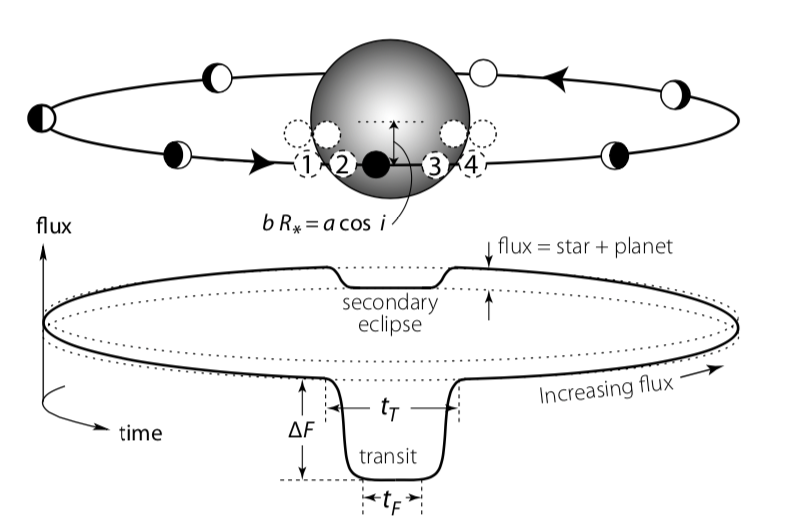
\includegraphics[width=0.8\columnwidth]{imagenes/transit.png}
\caption{Architecture of a transiting exoplanet.}
\label{transit}
\end{figure}

\begin{figure}[H]
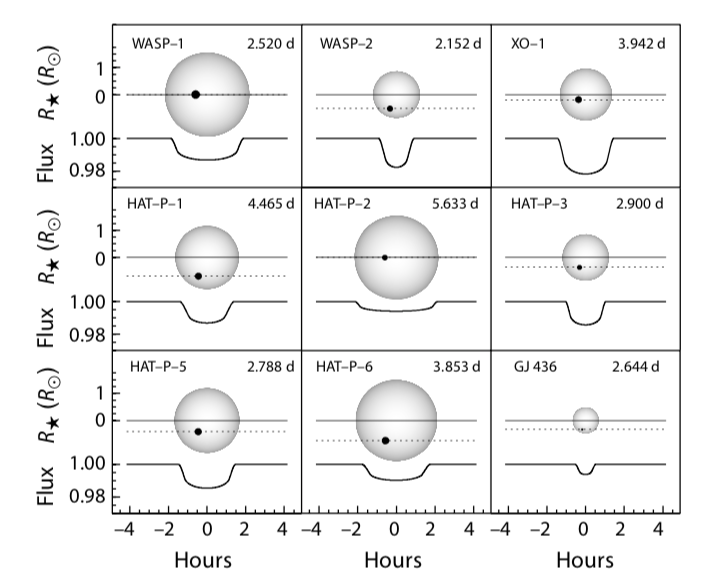
\includegraphics[width=1.0\columnwidth]{imagenes/transit_examples.png}
\caption{Examples of transiting exoplanets and how their light curves differ between them thanks to the physical properties of the exoplanet.}
\label{transit_examples}
\end{figure}



\section{Transit Timing Variations}

\section{The Transit Monitoring in the South project}% Introduccion
\chapter{Observations and Data Reduction}\label{chap:obs}

We collected 8 light curves for WASP-18b between 2009 and 2017, 9 light curves for WASP-19b between 2011 and 2017, and 5 light curves for WASP-77Ab between 2015 and 2017. We included 4 transits of WASP-77Ab from the Exoplanet Transit Database (ETD) in order to cover a larger timespan.

All of the photometry are collected by using either the Danish 1.54 m telescope at ESO La Silla Observatory, or the SMARTS 1 m at Cerro Tololo Observatory (CTIO), except for one transit of WASP-77Ab that was observed with the Warsaw 1.3 m at Las Campanas Observatory (LCO). The log of our observations is shown in Table XXX. All the new light curves used for this work are presented in Figure XXX.

For the photometric observations conducted on the Danish telescope, we used the Danish Faint Object Spectrograph and Camera (DFOSC) instrument, which has a $2{\rm K} \times 2{\rm K}$ CCD with a 13.7 x 13.7 arcmin$^2$ field of view (FoV) and a pixel scale of 0.39" per pixel. To reduce the readout time, some of the Danish 1.54 m images were windowed to only include the target star and its closest reference stars. The observations of the transits of WASP-18b during 2016 and 2017 were forced to be windowed due to a malfunction of the CCD. For those transits, only one reference star was used to perform the photometry.

The SMARTS 1 m has the Y4KCam instrument which is a $4{\rm K} \times 4{\rm K}$ CCD camera with a $20\times20$ arcmin$^2$ FoV and a pixel scale of 0.289" per pixel. 

For the observation on the Warsaw 1.3 m telescope, we used a $2048 \times 4096$ CCD camera chip with a 1.4 square degrees of FoV and 0.26" per pixel scale. No windowing or binning was used during the observations on both SMARTS 1m and the Warsaw 1.3m telescope.

As suggested by \cite{Southworth2009}, most of our observation, especially those conducted after 2011, used the defocus technique, which allows longer exposure times in bright targets and improves the photometric precision. We adjust the exposure time during the observations if the weather is not ideal. The recorded Julian Date in the Coordinated Universal Time (${\rm JD_{UTC}}$) were converted into Barycentric Julian Date in the Barycentric Dynamical Time standard (${\rm BJD_{TDB}}$) by following the procedure as in \citet{Eastman2010}.

We reduced the data by using our custom pipeline. It follows the standard procedures of reduction, calibration, and aperture photometry, but customized for each used instrument. The pipeline semi-automatically finds the best aperture and ring size, for the sky that produces the light curve with less RMS. Then, we manually choose the reference stars to produce the differential light curves for each targets.
\chapter{The case of WASP-18b}\label{chap:wasp18}

\section{The system}
WASP-18b is a transiting hot Jupiter discovered by \cite{Hellier2009} within the WASP-South transit survey \citep{Pollacco2006}. It is an extremely close-in planet orbiting a F6 type star with a period of 0.94 days. Regarding its physical properties, WASP-18b is about ten times more massive than Jupiter with approximately the same size ($M_{P}=10.3\,{\rm M_{Jupiter}}$, $R_{P}=1.1\,{\rm R_{Jupiter}}$). Even though a rapid orbital decay was predicted theoretically \citep{Hellier2009}, it is not observed yet \citep{Wilkins2017} and new theoretical models proposed a variation of less than 4 seconds in the transit time over a 20-yr baseline \citep{CollierCameron2018}. 

\section{Observations and Data Reduction}

\begin{table*}
\caption{Log of Observations}             
\label{log_table}      
\centering          
\begin{tabular}{cccccccc}
\hline\hline       
 Date & Epoch\footnotemark{a} & Telescope & Filter & Total exposures & Exposure time\footnotemark{b} & RMS\footnotemark{c} \\
 (UTC) &       &           &       &                   & (seconds) & (mmag)\\
\hline  
 2009 Oct 28 &-1904 & SMARTS 1 m & $I$ & 1412 & 1.5 & 8.49  \\
 2009 Oct 29 & -1903 & SMARTS 1 m & $I$ & 1435 & 2 & 5.67 \\
2009 Oct 30 & -1902 & SMARTS 1 m & $I$ & 1198 & 2  & 4.50 \\
 2011 Sep 06 & -1184 & SMARTS 1 m & $I$ & 203 & 15 & 2.40 \\
2016 Sep 24\footnotemark{d} & 776 & Danish 1.54 m & $I$ & 138 & 90 & 1.05  \\
2016 Sep 25\footnotemark{d} & 777 &Danish 1.54 m & $I$ & 159 & 90  & 0.96  \\
2016 Sep 26\footnotemark{d} & 778 & Danish 1.54 m & $I$ & 113 & 90 & 0.87  \\ \smallskip
2017 Sep 29\footnotemark{d} & 1169 & Danish 1.54 m & $R$ & 330 & 30 & 2.53 \\
\hline                  
\end{tabular}
\footnotetext{a}{The epoch 0 is $T_{0}$ in Tables , for WASP-18b, WASP-19b and WASP-77Ab, respectively.}
\footnotetext{b}{For the variable exposure times, we consider the average during the night.}
\footnotetext{c}{The RMS values were computed from the best fitted model of each light curve.}
\footnotetext{d}{Light curves obtained with only one reference star.}
\end{table*}


\section{Transit Parameters and Physical Properties}\label{transitparams}

The resulting parameters from the global fit of WASP-18 in comparison the with results of the discovery paper \cite{Hellier2009} and the most recent analysis with TESS data \citep{Shporer2018}, are listed in Table~\ref{wasp18}. While in \cite{Hellier2009} the analysis was performed combining photometry and RV data, in \cite{Shporer2018} only photometric data was used. 

%Stellar params
As the stellar spectroscopic priors were taken from the discovery paper \cite{Hellier2009}, our results for the stellar mass $M_*$ and radius $R_*$ are in good agreement with theirs, as expected, as well as the rest of the stellar parameters. \cite{Shporer2018} do not present results of stellar parameters.

%Primary transit params
In the case of the primary transit parameters, the greatest difference is found in the radius of the planet in stellar radii $R_{p}/R_{*}$. Our reported $R_{p}/R_{*}$ is $7.8\sigma$ and $4.4\sigma$ larger that the reported by \cite{Hellier2009} on the discovery paper and the recent result from \cite{Shporer2018}, respectively.  Our transit duration $T_{14}$ is also $3.4\sigma$ larger than the value from \cite{Hellier2009}.

% RV params
For the radial velocity parameters, the RV semi-amplitude derived from our analysis is consistent with the value of \cite{Hellier2009}, as the same data was used. 

% Derived params
Finally, the derived parameters of the system are, in general, in good agreement with the values from \cite{Hellier2009} and \cite{Shporer2018}. 

\begin{table*}
\caption{System parameter of WASP-18}
\label{wasp18}
\centering
\begin{tabular}{lcccc}
\hline \hline
~~~~Parameter & Units & This work & \cite{Hellier2009} & \cite{Shporer2018} \\
\hline
\smallskip\\\multicolumn{2}{l}{Stellar Parameters:}&\smallskip\\
~~~~$M_*$\dotfill &Mass (\(M_\odot\))\dotfill &$1.294^{+0.063}_{-0.061}$ & $1.25\pm0.13$ &  \\
~~~~$R_*$\dotfill &Radius (\(R_\odot\))\dotfill &$1.319^{+0.061}_{-0.062}$ &$1.26^{+0.067}_{-0.054}$ & \\
~~~~$L_*$\dotfill &Luminosity (\(L_\odot\))\dotfill &$2.68^{+0.28}_{-0.26}$ & &\\
~~~~$\rho_*$\dotfill &Density (cgs)\dotfill &$0.795^{+0.11}_{-0.089}$ & $ 0.707^{+0.056}_{-0.096}$&\\
~~~~$\log{g}$\dotfill & Surface gravity (cgs)\dotfill &$4.310^{+0.036}_{-0.033}$ &$4.367^{+0.028}_{-0.042}$ & \\
~~~~$T_{\rm eff}$\dotfill &Effective Temperature (K)\dotfill &$6432\pm48$ & $6400\pm100$& \\
~~~~$[{\rm Fe/H}]$\dotfill &Metallicity \dotfill &$0.107\pm0.080$ & $0.00\pm0.09$ & \\
~~~~$Age$\dotfill &Age (Gyr)\dotfill &$1.57^{+1.4}_{-0.94}$ & $0.5-1.5$ & \\
%~~~~$d$\dotfill &Distance (pc)\dotfill &$122.2^{+9.9}_{-8.2}$ & $100\pm10$ & \\

\smallskip\\\multicolumn{2}{l}{Planetary Parameters:}&\smallskip\\
~~~~$R_P$\dotfill &Radius (\rj)\dotfill &$1.310\pm0.071$ & $1.106^{+0.072}_{-0.054}$& $1.192\pm0.038$\\
~~~~$M_P$\dotfill &Mass (\mj)\dotfill &$10.48^{+0.42}_{-0.40}$ & $10.30\pm0.69$ & \\
~~~~$P$\dotfill &Period (days)\dotfill &$0.94145236\pm(49)$ & $0.94145299\pm(87)$& $0.9414576^{(+34)}_{(-35)}$ \\
~~~~$e$\dotfill &Eccentricity \dotfill &$0.0061^{+0.0089}_{-0.0044}$ & &\\
~~~~$a$\dotfill &Semi-major axis (AU)\dotfill &$0.02054^{+0.00033}_{-0.00032}$ & $0.02045\pm0.00067$&\\
~~~~$\omega_*$\dotfill &Argument of Periastron (Degrees)\dotfill &$-100^{+110}_{-120}$ &  &\\
~~~~$\rho_P$\dotfill &Density (cgs)\dotfill &$5.79^{+0.97}_{-0.78}$& $7.73^{+0.78}_{-1.27}$\footnotemark{b} & \\
~~~~$logg_P$\dotfill &Surface gravity \dotfill &$4.180^{+0.044}_{-0.041}$ & $4.289^{+0.027}_{-0.050}$ &\\
~~~~$T_{eq}$\dotfill &Equilibrium temperature (K)\dotfill &$2485^{+53}_{-56}$ & $2384^{+58}_{-30}$ & \\
~~~~$\Theta$\dotfill &Safronov Number \dotfill &$0.254^{+0.015}_{-0.014}$ & &\\
~~~~$\fave$\dotfill &Incident Flux (\fluxcgs)\dotfill &$8.66^{+0.77}_{-0.75}$ & & \\

\smallskip\\\multicolumn{2}{l}{Primary Transit Parameters:}&\smallskip\\
~~~~$T_0$\dotfill &Transit time (\bjdtdb)\dotfill &$2456740.80560\pm(19)$ & $2454221.48163\pm(38)$ & $2458361.048072^{(+34)}_{(-35)}$\\
~~~~$i$\dotfill &Inclination (Degrees)\dotfill &$83.5^{+2.0}_{-1.6}$ & $86.0\pm2.5$ & $84.31^{+0.40}_{-0.37}$\\
~~~~$R_P/R_*$\dotfill &Radius of planet in stellar radii \dotfill &$0.1021\pm0.0011$ &  $0.0935\pm0.0011$ & $0.09721^{+0.00016}_{-0.00017}$\\
~~~~$a/R_*$\dotfill &Semi-major axis in stellar radii \dotfill &$3.35^{+0.15}_{-0.13}$ & & $3.523^{+0.028}_{-0.027}$\\
~~~~$b$\dotfill &Impact parameter \dotfill &$0.433^{+0.07}_{-0.10}$ & $0.25\pm0.15$ & $0.349^{+0.020}_{-0.022}$\\
~~~~$\delta$\dotfill &Transit depth (fraction)\dotfill &$0.01041\pm0.00022$ & & $0.009449^{+0.000032}_{-0.000032}$\\
~~~~$u_{1,I}$\dotfill &linear LD coeff., I band\dotfill &$0.207\pm0.019$ & &\\
~~~~$u_{2,I}$\dotfill &quadratic LD coeff., I band\dotfill &$0.313\pm0.019$& &\\
~~~~$u_{1,R}$\dotfill &linear LD coeff., R band\dotfill & $0.257\pm0.045$ & &\\
~~~~$u_{2,R}$\dotfill &quadratic LD coeff., R band\dotfill &$0.309\pm0.048$ & &\\
~~~~$T_{14}$\dotfill &Total transit duration (days)\dotfill &$0.0931^{+0.0011}_{-0.0010}$ & $0.08932\pm0.00068$ &\\
~~~~$P_T$\dotfill &A priori non-grazing transit prob \dotfill &$0.268^{+0.011}_{-0.012}$ & &\\
~~~~$P_{T,G}$\dotfill &A priori transit prob \dotfill &$0.328^{+0.014}_{-0.015}$ & &\\
~~~~$\tau$\dotfill &Ingress/egress transit duration (days)\dotfill &$0.0107\pm0.0010$ & &\\

\smallskip\\\multicolumn{2}{l}{RV Parameters:}&\smallskip\\
~~~~$ecos{\omega_*}$\dotfill & \dotfill &$-0.0004^{+0.0038}_{-0.0045}$ & &\\
~~~~$esin{\omega_*}$\dotfill & \dotfill &$-0.0008^{+0.0056}_{-0.0092}$ & &\\
~~~~$K$\dotfill &RV semi-amplitude (m/s)\dotfill &$1807^{+34}_{-36}$ & $1818.3\pm8.0$ &\\
~~~~$M_P\sin i$\dotfill &Minimum mass (\mj)\dotfill &$10.40\pm0.40$ & &\\
\smallskip\\\multicolumn{2}{l}{Secondary Eclipse Parameters:}&\smallskip\\
~~~~$T_S$\dotfill &Time of eclipse (\bjdtdb)\dotfill &$2457657.3076^{+0.0023}_{-0.0027}$ & &\\
~~~~$b_S$\dotfill &Eclipse impact parameter \dotfill &$0.431^{+0.070}_{-0.100}$ & &\\
~~~~$\tau_S$\dotfill &Ingress/egress eclipse duration (days)\dotfill &$0.0106^{+0.0011}_{-0.0010}$ & &\\
~~~~$T_{S,14}$\dotfill &Total eclipse duration (days)\dotfill &$0.0929\pm0.0017$ & &\\
~~~~$P_S$\dotfill &A priori non-grazing eclipse prob \dotfill &$0.269^{+0.010}_{-0.011}$ & &\\
~~~~$P_{S,G}$\dotfill &A priori eclipse prob \dotfill &$0.330^{+0.013}_{-0.014}$ & &\\
\hline
\end{tabular}
%\tablefoot{
%\tablefoottext{a}{Value converted to cgs units multiplying by the Sun density $\rho_{\odot}=1.408\,$cgs.}
%\tablefoottext{b}{Value converted to cgs units multiplying by the Jupiter density $\rho_{J}=1.33\,$cgs.}
%\tablefoottext{c}{Values enclosed in parentheses correspond to the uncertainties of the last digits of the nominal value.}}
\end{table*}

\section{Transit Timing Variations}\label{ttvsection}

%\begin{figure*}
%\vspace{0cm}\hspace{0cm}
%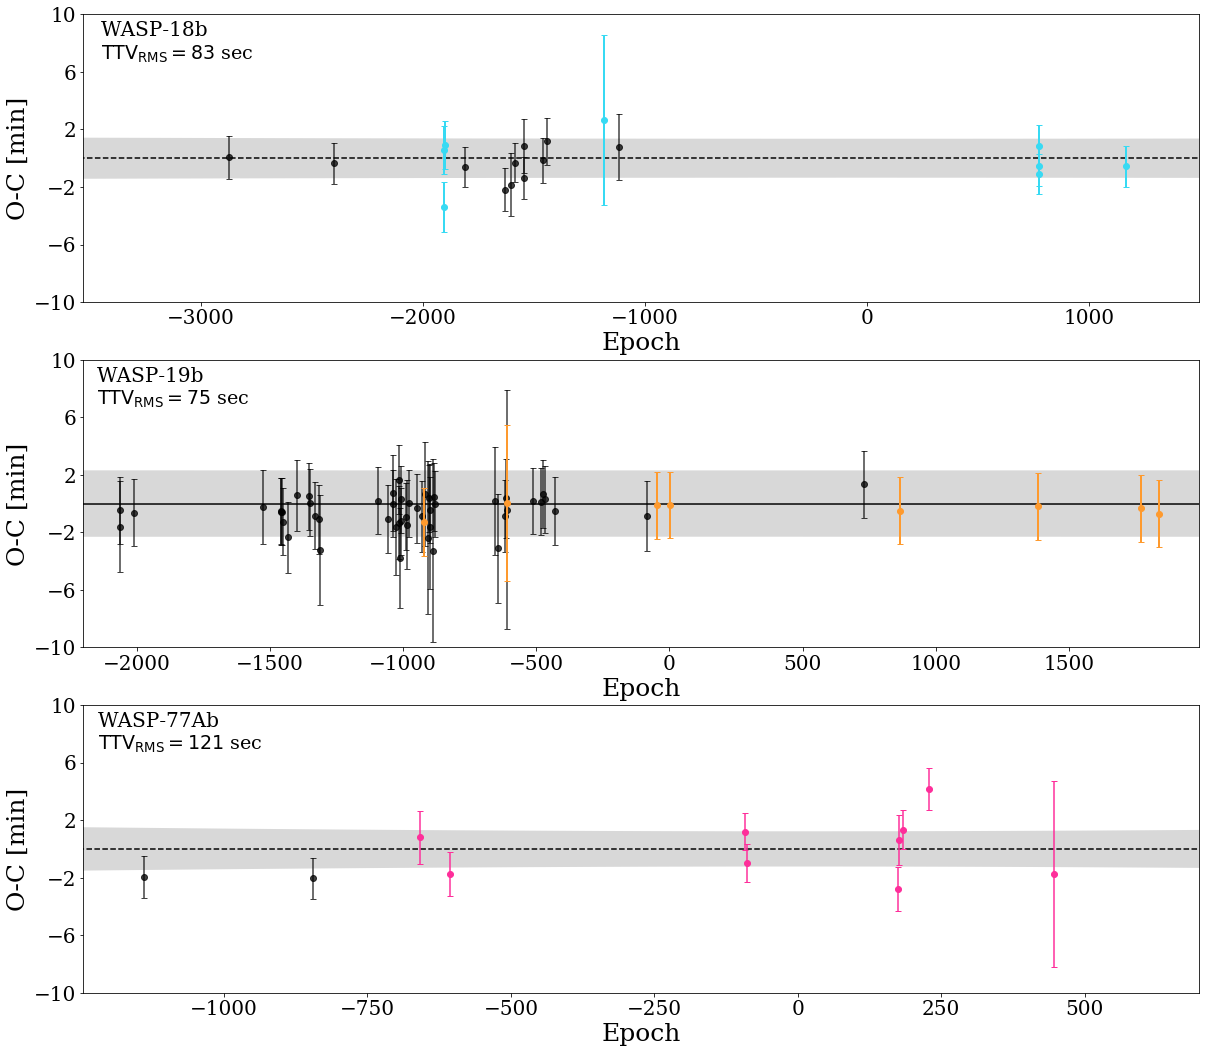
\includegraphics[width=1.0\textwidth]{TTVs.png}
%\centering
%\caption{Observed minus calculated mid-transit times (TTV) for WASP-18b (top), WASP-19b (center) and WASP-77Ab (bottom). The dashed black line corresponds to the proposed linear ephemeris, i.e. zero deviation from the predicted transit time (See Section \ref{ttvsection}) computed from our refined orbital period. For that, we considered 19, 59 and 11 transit times of WASP-18b, WASP-19b, and WASP-77Ab, respectively. The grey area corresponds to the error propagation at $1\sigma$, where the quadratic trend looks almost horizontal. The points in color are the TTV from the newly light curves of the TraMoS project (WASP-18b: light blue, WASP-19b: orange, WASP-77Ab: pink) and the black points in the three panels are TTVs measured from previous published transit times. The RMS scatter from the linear ephemeris are 83 seconds for WASP-18b; 75 seconds for WASP-19b, and 121 seconds for WASP-77Ab.}
%\label{ttv}
%\end{figure*}

For this system, the proposed linear ephemeris equation is:

\begin{equation} \label{eq1_w18}
T_{\rm C}(E)=2456926.27460\pm(94)+E \cdot 0.941452232\pm(89)
\end{equation}

The orbital period $P$ in Eq.~\ref{eq1_w18} is in complete agreement with the value computed only with the TraMoS light curves in Table~\ref{wasp18}.

Table~\ref{times_wasp18} lists the TTV of our transit times and also, of data from previous works \citep{Triaud2010,Hellier2009,Maxted2013b} of WASP-18b. 

The top panel of Figure... is the linear plot of TTV versus epoch for this planet. The deviations of the transit times from the linear ephemeris has an RMS of 83 seconds. The greater deviations come from the transit time of the epochs $-1904$ and $-1184$, which are over the linear ephemeris by $2.5\sigma$ and $1.9\sigma$, respectively. If those values are removed, the RMS decreases to 61 seconds. Considering all the transit times in Table~\ref{times_wasp18} without the epochs $-1904$ and $-1184$, all the TTVs lie within $1.6\sigma$ in the linear fit. 

The epoch $-1184$ has the greatest error in our sample because it is not a complete transit.

When testing the goodness of the linear fit, $\chi^{2}_{red} =0.56$, while for a second degree polynomial is $\chi^{2}_{red}=0.48$, therefore an orbital decay can be discarded in agreement with theoretical estimations \citep{CollierCameron2018}.  


\begin{table}
%\tablewidth{0pt}
\caption{Transit mid-times for WASP-18b}
\label{times_wasp18}
\begin{tabular}{cccc}
\hline \hline
Epoch & Transit mid-time & TTV & References\\
      & (${\rm BJD_{TDB}}$) & (min) & \\
\hline 
-2873 & $2454221.48238$ & $0.1\pm1.5$ & 1\\
-2402 & $2454664.9061$ & $-0.4\pm1.4$ & 2 \\
-1904 & $2455133.7472$ & $-3.4\pm1.7$ & This work \\
-1903 & $2455134.6914$ & $0.6\pm1.7$ & This work \\
-1902 & $2455135.6331$  & $0.9\pm1.7$  & This work \\
-1811 & $2455221.3042$ & $-0.6\pm1.4$  & 3\\
-1629 & $2455392.6474$ & $-2.2\pm1.5$& 3 \\
-1601 & $2455419.0083$ & $-1.8\pm2.2$& 3\\
-1587 & $2455432.1897$ & $-0.3\pm1.4$ & 3\\
-1546 & $2455470.7885$ & $-1.4\pm1.4$ & 3\\
-1543 & $2455473.6144$ & $0.9\pm1.9$& 3\\
-1457 & $2455554.5786$ & $-0.2\pm1.5$&3 \\
-1440 & $2455570.5842$ & $1.2\pm1.6$& 3\\
-1184 & $2455811.5970$ &  $2.7\pm5.9$ & This work  \\
-1115 & $2455876.5559$ & $0.8\pm2.3$ & 3 \\ 
776 & $2457656.84078$ & $-1.1\pm1.4$ & This work  \\
777 & $2457657.78359$   & $0.9\pm1.4$ & This work\\
778 & $2457658.72404$ & $-0.6\pm1.4$ & This work \\
1169 & $2458026.83186$ & $-0.6\pm1.5$ & This work  \\
\hline
\end{tabular}
%\tablebib{(1)~\citet{Hellier2009};
%(2) \citet{Triaud2010}; (3) \citet{Maxted2013}.}
\end{table} 

\subsection{Limits on an additional perturber}

For the WASP-18b system we find a large region of instability when compared to the other two systems with the boundaries at the 1:2 interior
and 2:1 exterior mean-motion resonance. By over-plotting the RMS scatter of mid-transit times ($\rm TTV_{\rm RMS}$) for a certain value, we find
that the TTVs are relatively more sensitive at orbital architectures involving mean-motion resonances confirming the results by \citet{Agol2005} and \citet{Holman2005}. %This also applies to WASP-19 and WASP-77A.

As shown in Figure~\ref{megno_wasp18}, we find that a perturbing body of mass (upper limit) around $7-500~M_{\oplus}$ will produce an RMS of $83\,{\rm s}$ when located in the $P_2/P_1=$ 7:3, 5:2, 3:1, 17:5 and 4:1 exterior resonance. For the 1:3 interior resonance, a perturber mass (upper limit) as small as $1.9~M_{\oplus}$ could also cause a RMS mid-transit time scatter of $83\,{\rm s}$.

\begin{figure}
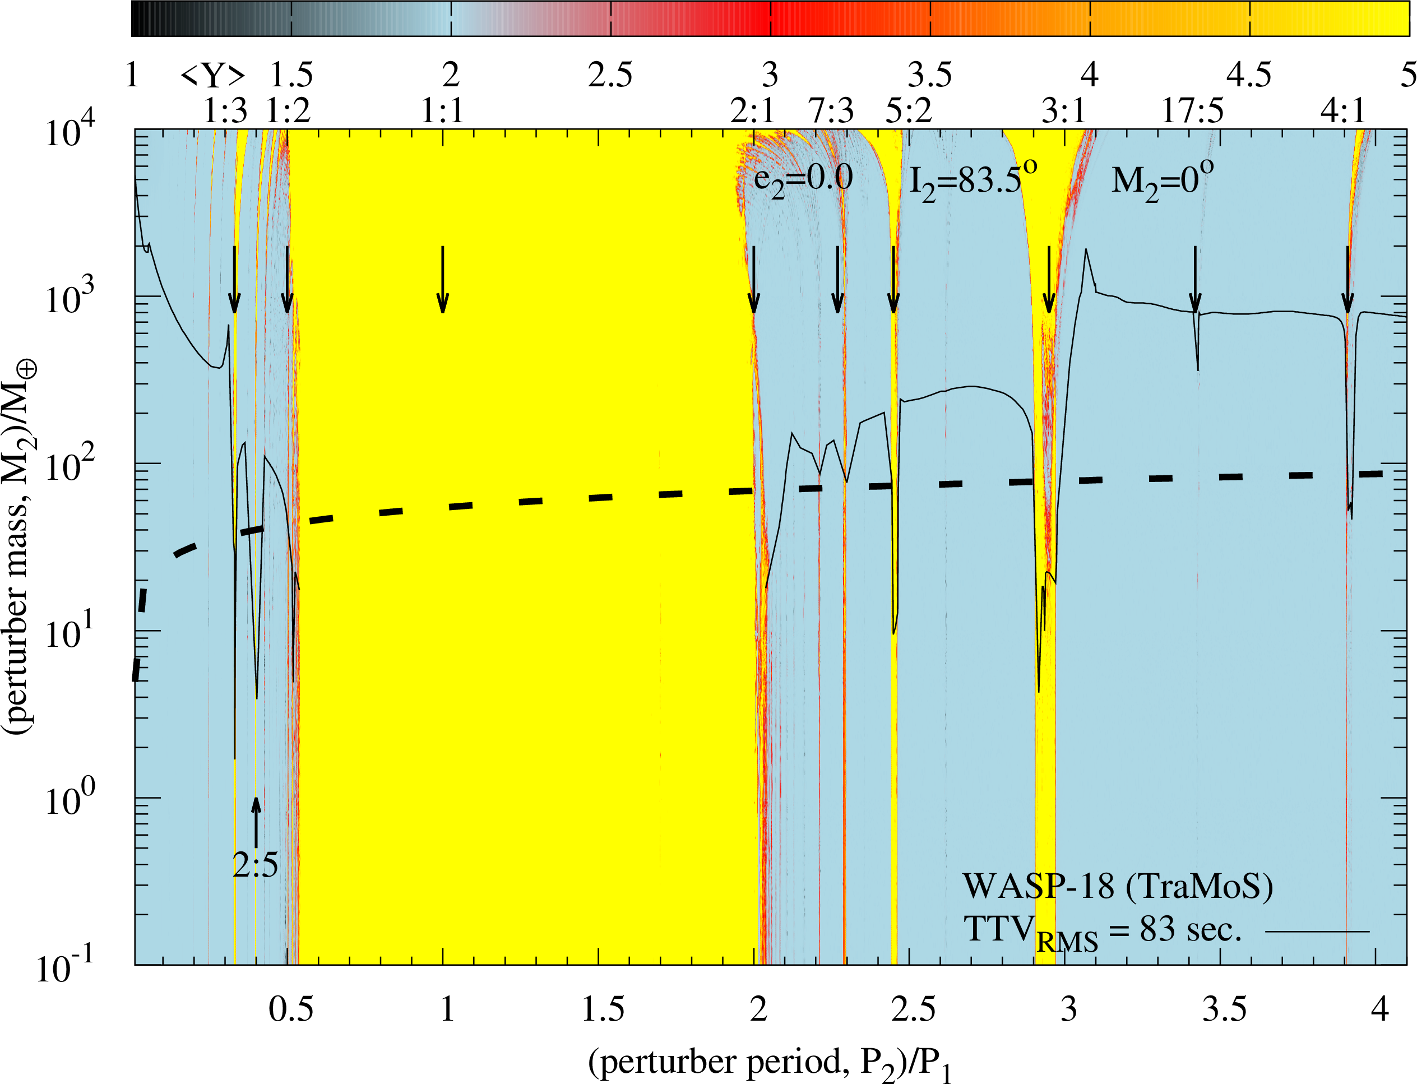
\includegraphics[width=1.0\columnwidth]{imagenes/WASP18_TraMos_83sec_Map001_GIMP_scaled.png}
\caption{MEGNO ($\langle Y \rangle$) stability map for the WASP-18 system. We over-plot the map with an upper mass of a hypothetical perturbing planet introducing a mid-transit time $\rm TTV_{\rm RMS}$ scatter of $83\,{\rm s}$ (solid line) as obtained in this study. The stipulated line is the upper mass limit as obtained from the RMS scatter $(30.9\, \rm m/s)$ of the radial-velocity curve. For initial conditions resulting in a quasi-periodic (i.e bounded) motion of the system, the $\langle Y\rangle$ value is close to 2.0 (color coded blue). For chaotic (i.e unstable) motion, the $\langle Y \rangle$ is diverging away from 2.0 (color coded red to yellow). Vertical arrows indicate $(P_2/P_1)$ orbital resonances between the perturbing body and the transiting planet. The two planets were assumed to be co-planar, and the perturbing planet's eccentricity was initially set to zero.
\emph{See electronic version for colors}.}
\label{megno_wasp18}
\end{figure}
\chapter{The case of WASP-19b}\label{chap:wasp19}

\section{The system}

\section{Transit Parameters and Physical Properties}

\section{Transit Timing Variations}

\section{Limits on an additional perturber}
\chapter{The case of WASP-77Ab}\label{chap:wasp77}
%\input{chap_teoria.tex}		% Marco teórico
%\input{chap_nao_backpack.tex}% Sistema General
%\input{chap_slam_visual.tex}	% Sistema General
%\input{chap_odometria.tex}	% Sistema General
%\input{chap_resultados.tex}	% Resultados
%\input{chap_conclusiones.tex}% Conclusiones

% ----------------------------------------------------------------------
% Glosario
% ----------------------------------------------------------------------
%\input{glosario.tex} % opcional

% ----------------------------------------------------------------------
% Bibliografía
% ----------------------------------------------------------------------

\addcontentsline{toc}{chapter}{Bibliography}
\bibliographystyle{apa}
{\small
\bibliography{references}
}

% ----------------------------------------------------------------------
% Apéndice
% ----------------------------------------------------------------------

%\begin{appendices}
%\input{apendice_nao_datasheet.tex} 	     % especificaciones del NAO
%\input{apendice_setup_experimental.tex}  % setup experimental
%\input{apendice_lie.tex} 	             % grupos de Lie
%\input{apendice_intentos.tex}	         % Lo que se intentó y no funcionó
%\input{apendice_imu.tex}	             % derivacion de modelo cinemático de la IMU
%\input{apendice_agradecimientos.tex}	 % agradecimientos
%\end{appendices}

\end{document}
\grid
